\documentclass[10pt,twocolumn,letterpaper]{article}

\usepackage{times}
\usepackage{graphicx}
\usepackage{amsmath}
\usepackage{amssymb}
\usepackage{caption}
\usepackage{color}
\usepackage{subfig}
\usepackage{lipsum}

\usepackage[pagebackref=true,breaklinks=true,letterpaper=true,colorlinks,bookmarks=false]{hyperref}

  
\newcommand{\shortcite}[1]{\cite{#1}}
\newcommand{\ignorethis}[1]{}
\def\httilde{\mbox{\tt\raisebox{-.5ex}{\symbol{126}}}}



% set dimensions of columns, gap between columns, and paragraph indent
\setlength{\textheight}{8.9in}
\setlength{\textwidth}{7in}
\setlength{\columnsep}{0.3125in}
\setlength{\topmargin}{0in}
\setlength{\headheight}{0in}
\setlength{\headsep}{0in}
\setlength{\parindent}{1pc}
\setlength{\oddsidemargin}{-.25in}
\setlength{\evensidemargin}{-.25in}
 
 

\begin{document}



\title{Title: Machine Learning.....}

\author{
First Name Last Name\thanks{empty}
\and
First Name Last Name\footnotemark[1]
\and 
First Name Last Name
\and
Department of Mathematics, Northeastern University
}



\twocolumn[{%
\renewcommand\twocolumn[1][]{#1}%

\maketitle
}]


\begin{abstract}
 
\textit{Image-to-image translation is a class of vision and graphics problems where the goal is to learn the mapping between an input image and an output image using a training set of aligned image pairs.   
However, for many tasks, paired training data will not be available.  We present an approach for learning to translate an image from a source domain $X$ to a target domain $Y$ in the absence of paired examples.  Our goal is to learn ...}
\end{abstract}

 


% New section
\section{Introduction}
 \label{Intro: }

 

We can imagine all this despite never having seen a side by side example of a Monet painting next to a photo of the scene he painted. Instead, we have knowledge of the set of Monet paintings and of the set of landscape photographs. We can reason about the stylistic differences between these two sets, and thereby imagine what a scene might look like if we were to ``translate'' it from one set into the other.

In this paper, we present a method that can learn to do the same: capturing special characteristics of one image collection and figuring out how these characteristics could be translated into the other image collection, all in the absence of any paired training examples. 
 
 ...
 
% New section
\section{Related work}
 

 

{\bf Image-to-Image Translation}
The idea of image-to-image translation goes back at least to Hertzmann et al.'s Image Analogies~\cite{hertzmann2001image}, who employ a non-parametric texture model~\cite{efros1999texture} on a single input-output training image pair.
More recent approaches use a \emph{dataset} of input-output examples to learn a parametric translation function using CNNs (e.g.,~\cite{long2015fully}). 

Our approach builds on the ``pix2pix" framework of Isola et al.~\cite{isola2016image}, which uses a conditional generative adversarial network~\cite{goodfellow2014generative} to learn a mapping from input to output images. Similar ideas have been applied to various tasks such as generating photographs from sketches~\cite{sangkloy2016scribbler} or from attribute and semantic layouts~\cite{karacan2016learning}. However, unlike the above prior work, we learn the mapping without paired training examples. 

....


\begin{figure}
 \centering
 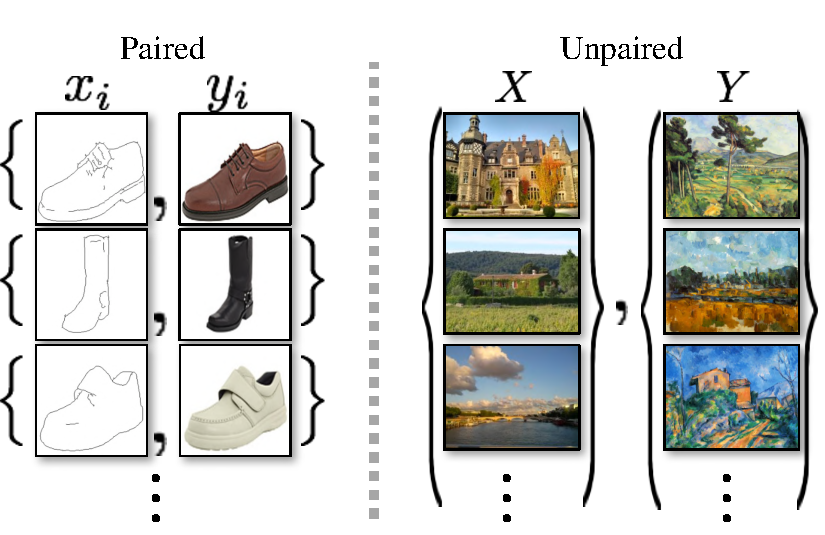
\includegraphics[width=1.0\hsize]{paired_unpaired2.pdf}
 \vspace{-0.3in}
  \caption{\emph{Paired} training data (left)  ...}
 \vspace{-0.2in}
\end{figure}

% New section
\section{Formulation}
 


Our goal is to learn mapping functions between two domains $X$ and $Y$ given training samples $\{x_i\}_{i=1}^N$ where $x_i \in X$ and $\{y_j\}_{j=1}^M$  

\subsection{Adversarial Loss}
We apply adversarial losses~\cite{goodfellow2014generative} to both mapping functions.  
...


% New section
\section{Implementation}
 

\paragraph{Network Architecture}
We adopt the architecture for our generative networks from Johnson et al.~\shortcite{johnson2016perceptual} who have shown impressive results for neural style transfer and super-resolution. This network contains three convolutions,  
...


\section{Results}
 
We first compare our approach against recent methods for unpaired image-to-image translation on paired datasets where ground truth input-output pairs are  
 

\subsubsection{Comparison against baselines}
As can be seen in  ? and  ?, we were unable to achieve compelling results with any of the baselines. Our method, on the other hand, can produce ...

 
...
 
 \section{Acknowledgement}
We would like to thank ... for providing the data. ...
 
 
 

\bibliographystyle{ieee}

\begin{thebibliography}{10}\itemsep=-1pt

\bibitem{aytar2016cross}
Y.~Aytar, L.~Castrejon, C.~Vondrick, H.~Pirsiavash, and A.~Torralba.
\newblock Cross-modal scene networks.
\newblock {\em PAMI}, 2016.

\bibitem{bousmalis2016unsupervised}
K.~Bousmalis, N.~Silberman, D.~Dohan, D.~Erhan, and D.~Krishnan.
\newblock Unsupervised pixel-level domain adaptation with generative
  adversarial networks.
\newblock In {\em CVPR}, 2017.


\bibitem{bousmalis2016unsupervised}
...

\end{thebibliography}


\end{document}
